\documentclass[12pt, letterpaper]{article}

\setlength {\marginparwidth }{2cm}

\usepackage{tikz}
\usetikzlibrary{shapes,arrows}
\tikzstyle{line}=[draw]
\usepackage{amsthm}
\usepackage{amsmath}
\usepackage[textsize=tiny]{todonotes}

%\newtheorem{thm}{Theorem}
%\newtheorem{defn}[thm]{Definition}

%% commands taken from Adam Petz's submission to NFM in 2021 

\newtheorem{thm}{Theorem}
\newtheorem{lem}[thm]{Lemma}
\newtheorem{defn}[thm]{Definition}
\newtheorem{ex}[thm]{Example}
%\newtheorem{claim}[thm]{Claim}

%\newcommand{\squash}{\parskip=0ex\itemsep=0ex}
\newcommand{\cnf}[1]{\ensuremath{\operatorname{\mathsf{#1}}}}
\newcommand{\cnc}[1]{\ensuremath{\mathsf{#1}}}
\newcommand{\fnf}[1]{\ensuremath{\operatorname{\mathit{#1}}}}
\newcommand{\fnc}[1]{\ensuremath{\mathit{#1}}}

% Binary operators for linear and branching terms
\newcommand{\linseq}{\prec}
\newcommand{\linpar}{\sim}
\newcommand{\sdup}{\leftrightarrow}
\newcommand{\slft}{\leftarrow}
\newcommand{\srht}{\rightarrow}
\newcommand{\bradupseq}{\stackrel{\sdup}{\linseq}}
\newcommand{\bralftseq}{\stackrel{\slft}{\linseq}}
\newcommand{\brarhtseq}{\stackrel{\srht}{\linseq}}
\newcommand{\braduppar}{\stackrel{\sdup}{\linpar}}
\newcommand{\bralftpar}{\stackrel{\slft}{\linpar}}
\newcommand{\brarhtpar}{\stackrel{\srht}{\linpar}}
\newcommand{\linseqe}{\to}
\newcommand{\braseqe}[1]{\stackrel{#1}{\prec}}
\newcommand{\brapare}[1]{\stackrel{#1}{\sim}}

\newcommand{\apdt}{APDT}
\newcommand{\skp}{\cnc{SKIP}}
\newcommand{\cpy}{\cnc{CPY}}
\newcommand{\done}{\cnc{DONE}}
\newcommand{\at}[2]{\mathop{@_{#1}}{#2}}
%\newcommand{\ati}[3]{\mathop{@_{#1}}[{#2}]{#3}}
\newcommand{\sig}{\cnc{SIG}}
\newcommand{\hsh}{\cnc{HSH}}
\newcommand{\kimc}{\cnc{KIM}}
\newcommand{\kim}[3]{\cnc{KIM}~#1~#2~#3}
\newcommand{\kime}[3]{\cnc{KIM}~#1~#2~#3}
\newcommand{\usm}{\cnc{USM}}
\newcommand{\usme}[2]{\cnc{USM}~#1~#2}

\newcommand{\aspev}{\cnc{ASP}}
\newcommand{\aspn}{\cnc{ASP}}

\newcommand{\aspt}[2]{\cnc{ASP}~#1~#2}
\newcommand{\asptn}[4]{\cnc{ASP}~#1~#2~#3~#4}
\newcommand{\aspe}[4]{\cnc{U}~#1~#2~#3~(#4)}
\newcommand{\aspenn}[2]{\cnc{U}~#1~(#2)}
\newcommand{\aspen}[2]{\cnc{U}~#1~#2}
\newcommand{\Ge}[2]{\cnc{G}~#1~#2}
\newcommand{\He}[1]{\cnc{H}~#1}
\newcommand{\nidt}{\cnc{n}}
\newcommand{\nid}{\emph{nonce\_id}}
\newcommand{\bits}{\emph{bits}}
\newcommand{\plc}{\emph{place\_id}}
\newcommand{\aspid}{\emph{asp\_id}}
\newcommand{\Net}[3]{\cnc{N}~{#1}~#2~#3}
%\newcommand{\Nett}[3]{\cnc{N}~{#1}~#2~(#3)}

\newcommand{\aspet}[4]{\cnc{U_t}~#1~#2~#3~(#4)}
\newcommand{\Get}[2]{\cnc{G_t}~#1~#2}
\newcommand{\Het}[1]{\cnc{H_t}~#1}
\newcommand{\Nett}[2]{\cnc{N_t}~{#1}~#2}


\newcommand{\seqe}{\mathbin{;\!;}}
\newcommand{\pare}{\parallel}
\newcommand{\mt}{\xi}
\newcommand{\sign}[2]{[\![#1]\!]_{#2}}
\newcommand{\hash}[2]{\mathop{\#_{#1}}{#2}}
\newcommand{\KK}[2]{\cnc{K}^{#1}_{#2}}
\newcommand{\UU}[1]{\cnc{U}_{#1}}
\newcommand{\Ke}[4]{\cnc{K}^{#1}_{#3}({#4})}
\newcommand{\Ue}[3]{\cnc{U}_{#2}({#3})}
\newcommand{\UUU}[2]{\cnc{U}_{#1}({#2})}
\newcommand{\Ne}[2]{\cnc{N}_{#1}({#2})}

\newcommand{\eval}[3]{\mathcal{E}({#1},{#2},{#3})}
\newcommand{\aeval}[3]{\bar{\mathcal{E}}({#1},{#2},{#3})}
\newcommand{\evalS}[1]{\ensuremath{\mathcal{E}(#1)}}
\newcommand{\evalv}[3]{\mathcal{V}({#1},{#2},{#3})}
%\newcommand{\evalv}[2]{\mathcal{V}({#1},{#2})}
\newcommand{\evalvS}[1]{\mathcal{V}({#1})}
\newcommand{\po}[3]{\mathcal{R}({#1},{#2},{#3})}
\newcommand{\bfr}[3]{{#1}\mathbin:{#2}\prec{#3}}
%\newcommand{\bfr}[3]{{#2}\prec_{#1}{#3}}
\newcommand{\splt}[2]{\mathcal{S}({#1},{#2})}
\newcommand{\subterm}{\sqsubseteq}
\newcommand{\sevalf}{\mathcal{F}}
\newcommand{\seval}[1]{\sevalf({#1})}
\newcommand{\placef}{\mathcal{G}}
\newcommand{\place}[1]{\placef({#1})}
\newcommand{\halt}[1]{\mathcal{H}({#1})}
\newcommand{\size}[1]{|{#1}|}
\newcommand{\evof}{\mathrel\Diamond}
\newcommand\te[4]{{#1}\evof^{#2}_{#3}{#4}}
% for tables
\newcommand\tte[4]{{#1}&{}\evof^{#2}_{#3}{}&{#4}}

\newcommand{\futr}{\cnc{FUTR}}

\newcommand{\nat}{\mathbb{N}}
\newcommand{\anno}[3]{[{#1}]^{#2}_{#3}}
\newcommand{\step}{\leadsto}
\newcommand{\lts}[3]{{#2}\mathbin:{#1}\step{#3}}
\newcommand{\lstp}[3]{{#1}\stackrel{#2}{\leadsto}{#3}}
\newcommand{\nstep}[1]{\leadsto^{{}_{#1}}}
\newcommand{\kstar}{\leadsto^*}
\newcommand{\nlstep}[2]{\stackrel{\!\!#1}{\leadsto^{{}_{#2}}}}
\newcommand{\lstep}[1]{\stackrel{#1}{\leadsto}}
\newcommand{\lstar}[1]{\stackrel{\!\!#1}{\leadsto^{{}_{*}}}}
\newcommand{\nlstar}[2]{\stackrel{\!\!#1}{\leadsto^{{}_{#2}}}}
\newcommand{\sseq}{\mathbin{;}}
\newcommand{\sfut}{\mid}
\newcommand{\qmid}{\mathbin{\mbox{`$\mid$'}}}
\newcommand{\ssft}{\mathbin{;\!;}}
\newcommand{\spar}{\parallel}
\newcommand{\sstop}{\mathcal{D}}
\newcommand{\conf}{\mathcal{C}}
\newcommand{\lseq}{\mathcal{LS}}
\newcommand{\bseq}{\mathcal{BS}}
\newcommand{\bpar}{\mathcal{BP}}
\newcommand{\ats}{\mathcal{A}}

\newcommand{\compf}{\mathcal{C}}
\newcommand{\comp}[2]{\compf({#1},{#2})}
\newcommand{\compp}[2]{[{#2}]_{#1}}
\newcommand{\cop}[1]{\mathbin{\cdot{#1}\cdot}}
\newcommand{\atc}[1]{\mathop{\bar{@}_{#1}}}
\newcommand{\estep}{\Rightarrow}

\newcommand{\seq}[1]{\ensuremath{\langle#1\rangle}}
%\newcommand{\app}{\mathbin{{}^\smallfrown}}
\newcommand{\app}{\mathbin{\ast}}
\newcommand{\cons}{\mathbin{::}}
\newcommand{\sel}{\mathbin{\downarrow}}

\newcommand{\csize}[1]{\ensuremath{\mid\!#1\!\mid}}
\newcommand{\labi}[2]{\ensuremath{\alpha({#1},#2)}}
\newcommand{\lab}[1]{\ensuremath{\alpha(#1)}}
%\newcommand{\tsize}[1]{\ensuremath{\mid\!#1\!\mid}}
\newcommand{\tsize}[1]{\size{#1}}

\newcommand{\term}{\cnc{APDT}}
%\newcommand\tr[4]{{#1}\mathcal{T}^{#2}_{#3}{#4}}
\newcommand\tr[4]{{#1}\mathbin\Box^{#2}_{#3}{#4}}
\newcommand{\trace}[2]{\ensuremath{\mathcal{T}(#1,#2)}}
\newcommand{\traceS}[2]{\ensuremath{\mathcal{T}(#1,#2)}}


\newcommand{\utype}[3]{\cnc{(\forall#1<:#2.\hspace{1mm} #3)}}
\newcommand{\tyu}[2]{\cnc{(\forall#1.\hspace{1mm} #2)}}
\newcommand{\uterm}[3]{\cnc{(\lambda#1<:#2.\hspace{1mm} #3)}}
\newcommand{\nilenv}[0]{$\emptyset$}
\newcommand{\topt}{\cnc{TOP}}
\newcommand{\noncec}{\cnc{NONCE}}
\newcommand{\lam}[3]{\cnc{(\lambda}#1:#2 . \hspace{1mm} #3)}
\newcommand{\tylam}[2]{\cnc{(\lambda}#1 . \hspace{1mm} #2)}
\newcommand{\typest}[0]{\cnc{T} }
\newcommand{\id}[0]{\cnc{\emph{x}} }
\newcommand{\tid}[0]{\cnc{\emph{X}} }
\newcommand{\appl}[2]{#1 \hspace {2mm} #2}
\newcommand{\tappl}[2]{#1 \hspace {2mm} [#2]}
\newcommand{\terms}[0]{\cnc{\emph{t}} }
\newcommand{\meast}[0]{\cnc{MEAS}}
\newcommand{\evt}[0]{\cnc{\emph{E}} }
\newcommand{\evc}[0]{\cnc{\emph{e}} }
\newcommand{\evct}[0]{\cnc{\emph{e}_t} }
\newcommand{\arrt}[2]{#1 \hspace{1mm} \cnc{\rightarrow} \hspace{1mm} #2}
\newcommand{\pl}[0]{\cnc{\emph{P}} }
\newcommand{\placec}[1]{\cnc{pl_#1}}
\newcommand{\placee}[1]{\cnc{PL_#1}}
\newcommand{\placet}[0]{\cnc{PLACE_Q}}
% \DeclareMathOperator{\vvdash}{\vdash}
% \newcommand{\typeof}[3]{\cnc{\Gamma \vvdash\limits_{#1,#2} : #3}}
\newcommand{\btt}[2]{\cnc{(#1,#2)} \hspace{1mm} \ensuremath{\epsilon\hspace{1mm}\Gamma}}
\newcommand{\bs}{\cnc{bs}}
\newcommand{\argt}{\cnc{ARG}}
\newcommand{\Uec}[5]{\cnc{U}_{#1}~#2~#3~#4~(#5)}
\newcommand{\Kec}[6]{\cnc{K}^{#1}_{#2}~#3~#4~#5~(#6)}
\newcommand{\Gec}[3]{\cnc{G}_{#1} \hspace{1mm} #2 \hspace{1mm}  #3}
\newcommand{\Hec}[2]{\cnc{H}_{#1} \hspace{1mm} #2}
\newcommand{\Nec}[3]{\cnc{N}_{#1} \hspace{1mm} #2 \hspace{1mm} (#3)}
\newcommand{\Sec}[2]{\cnc{SS} \hspace{1mm} {#1} \hspace{1mm} {#2}}
\newcommand{\Pec}[2]{\cnc{PP} \hspace{1mm} {#1} \hspace{1mm} {#2}}
\newcommand{\mtc}{\cnc{mt}}
\newcommand{\mtct}{\cnc{mt_t}}
\newcommand{\strj}{\cnc{<string>}}
\newcommand{\numj}{\cnc{<number>}}
\newcommand{\arrj}{\cnc{<array>}}
\newcommand{\tj}{\cnc{<term>}}
\newcommand{\ej}{\cnc{<evidence>}}
\newcommand{\namej}{\cnc{<nameMap>}}
\newcommand{\reqmc}[5]{#1~#2~#3~#4~#5}
\newcommand{\respmc}[4]{#1~#2~#3~#4}


\newcommand{\Sect}[2]{\cnc{SS_t} \hspace{1mm} {#1} \hspace{1mm} {#2}}
\newcommand{\Pect}[2]{\cnc{PP_t} \hspace{1mm} {#1} \hspace{1mm} {#2}}

\newcommand{\squash}{\itemsep=0pt\parskip=0pt}

\title{Context Relation Musings}
\author{Anna Fritz}
\date{\today}

\begin{document}

\maketitle

\section{Context Defined}

First, in order to do any real reasoning about a system's context, we must formally define it. 

\begin{defn}[Context]
  A system's \emph{context} is a relationship represented within a Manifest that describes the dependencies within the system. 
\end{defn}

Some questions and interesting points arise when attempting to grasp this definition and realize the following example. Below are some words I think we need to define as we work towards the ordering problem. 

\begin{defn}[Dependency] 
  One component \emph{depends} on another when... 
\end{defn}

\begin{defn}[Similar] 
  One protocol is \emph{similar} to another when... They measure the same targets? The measurement chain reaches the same depth? The measurement chain reaches the same range? 
\end{defn}

\begin{defn}[Better] 
  One protocol is \emph{better} than another when... 
\end{defn}

\section{Example System}

Consider the example presented in Figure \ref{fig:Host1} where a request is sent to a target $Host1$. We know a request is a list of protocols as Copland phrases. Let's assume that $R$ = [ $\at{Host1}{} $ (ASP Host2 t2) ] which says some relying party would like the target system to preform a measurement of the target $T2$ located on $Host2$. 

The arrow between ASP and T2 reveals that ASP can measure T2. This results in the following Copland phrase: 

\begin{center}
  $ \at{Host1} (ASP\:\: Host2\:\: T2)$
\end{center}

\begin{figure}[]
  \centering 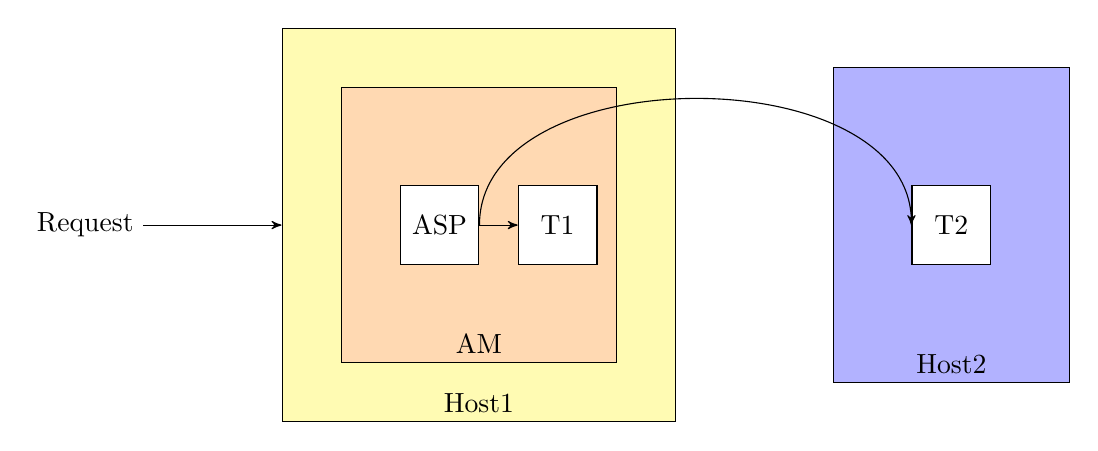
\begin{tikzpicture}[->,>=stealth']

      \node (req) at (-8,0) {Request};
  
      \node[rectangle,
            draw,
            fill = yellow!30,
            minimum width = 5cm, 
            minimum height = 5cm] (r) at (-3,0) {};
      \node[anchor=south] at (r.south) {Host1};
      
      \node[rectangle,
            draw,
            fill = orange!30,
            minimum width = 3.5cm, 
            minimum height = 3.5cm] (AM) at (r.center) {};
      \node[anchor=south] at (AM.south) {AM}; 

      \node[rectangle,
            draw,
            fill = white,
            minimum width = 1cm, 
            minimum height = 1cm] (ASP) at (-3.5,0) {};
      \node at (ASP.center) {ASP};

      \node[rectangle,
            draw,
            fill = white,
            minimum width = 1cm, 
            minimum height = 1cm] (T1) at (-2,0) {};
      \node at (T1.center) {T1};

      \node[rectangle,
            draw,
            fill = blue!30,
            minimum width = 3cm, 
            minimum height = 4cm] (Host2) at (3,0) {};
      \node[anchor=south] at (Host2.south) {Host2}; 

      \node[rectangle,
            draw,
            fill = white,
            minimum width = 1cm, 
            minimum height = 1cm] (T2) at (3,0) {};
      \node at (T2.center) {T2};
      

      \path[every node/.style={font=\sffamily\small}]
      (req) edge node [right] {} (r.west)
      (ASP.east) edge node [right] {} (T1.west)
      (ASP.east) edge[bend left = 90] node [left] {} (T2.west);

      % \draw (ASP.east) -- (T1.west); 
      % \draw [bend right] (ASP.east) -- (T2.west); 
  
  \end{tikzpicture}
  \caption{Example Target System.}
  \label{fig:Host1}
\end{figure}

For examples sake, say that ASP no longer has direct access to the measurement target T2 yet the goal of the attestation was to measure T2. This means we will have to realize a measurement of T2 is a different way. To start, we can expand Host2 to get a view of its attestation capabilities. This is represented with Figure \ref{fig:Host2}. We see Host2 has some ASP, $ASP2$ which can preform a measurement of $T2$. The integrity of the measurer $ASP2$ depends on the integrity of the following components: the operating system (OS), the device driver (DR), and some cryptographic operations $ \{ \}_{K}$. Then, these components all depend on the integrity of the root of trust measurement (RoTM). These dependencies are represented within Host2's manifest. 

In an abstract-ish version of Copland, the measurement chain for HOST2 could look like: 

\begin{center}
  $ \at{Host2}{(ROTM \linseqe ( OS \brapare{} DR \brapare{} \{ \}_{K} ) \linseqe (ASP2\:\: Host2\:\: T2))}$
  \todo{I have no idea how to use parathesis and Copland...}
\end{center}

where $\linseqe$ represents sequenced measurement and $\brapare{}$ represents parallel measurement. In other words, this phrase says, measure the root of trust, then measure OS, DR, and $\{ \}_{K}$ in parallel, then finally use ASP2 to take a measurement of T2. 

\todo{To be technically correct, how do you phrase the relationship between OS, DR, and SIG and the ROTM?}

\begin{figure}[]
  \centering 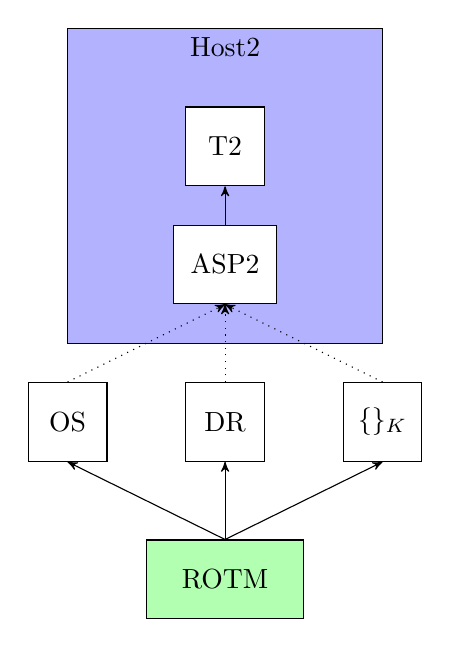
\begin{tikzpicture}[->,>=stealth']

    \node[rectangle,
          draw,
          fill = blue!30,
          minimum width = 4cm, 
          minimum height = 4cm] (Host2) at (0,0) {};
    \node[anchor=north] at (Host2.north) {Host2}; 

    \node[rectangle,
          draw,
          fill = white,
          minimum width = 1cm, 
          minimum height = 1cm] (T2) at (0,.5) {};
    \node at (T2.center) {T2};

    \node[rectangle,
        draw,
        fill = white,
        minimum width = 1.3cm, 
        minimum height = 1cm] (ASP2) at (0,-1) {};
    \node at (ASP2.center) {ASP2};

    \node[rectangle,
        draw,
        fill = white,
        minimum width = 1cm, 
        minimum height = 1cm] (OS) at (-2,-3) {};
    \node at (OS.center) {OS};

    \node[rectangle,
        draw,
        fill = white,
        minimum width = 1cm, 
        minimum height = 1cm] (DR) at (0,-3) {};
    \node at (DR.center) {DR};

    \node[rectangle,
        draw,
        fill = white,
        minimum width = 1cm, 
        minimum height = 1cm] (SIG) at (2,-3) {};
    \node at (SIG.center) {$ \{ \}_{K}$};

    \node[rectangle,
        draw,
        fill = green!30,
        minimum width = 2cm, 
        minimum height = 1cm] (RoTM) at (0,-5) {};
    \node at (RoTM.center) {ROTM};
    

    \path[every node/.style={font=\sffamily\small}]
    (ASP2.north) edge node [left] {} (T2.south)
    (OS.north) edge [dotted] node {} (ASP2.south)
    (DR.north) edge [dotted] node {} (ASP2.south)
    (SIG.north) edge [dotted] node {} (ASP2.south)
    (RoTM.north) edge node {} (OS.south)
    (RoTM.north) edge node {} (DR.south)
    (RoTM.north) edge node {} (SIG.south);

\end{tikzpicture}
  \caption{Example Host2 System.}
  \label{fig:Host2}
\end{figure}

For examples sake, say that ASP no longer has access to the measurement of T2 directly yet the goal of the attestation is to measure T2. Combining Host1 and Host2 and representing this new fact, we have the following system in Figure \ref{fig:System1}. If the request remains \\  $R$ = [ (ASP Host2 T2) ] we must consider what would be a ``similar'' measurement? This idea captures the concept of ordering measurements using the \emph{measures} and \emph{context} relations. 

\todo{define similar?}

\pagebreak
Say we have the following protocol, as would be represented in Figure \ref{fig:Host1} and Figure \ref{fig:Host2}.

\begin{eqnarray*}
  P1 &=& \at{Host1} (ASP\:\: Host2\:\: T2) \\
  P2 &=& \at{Host2}{(ROTM \linseqe ( OS \brapare{} DR \brapare{} \{ \}_{K} ) \linseqe (ASP2\:\: Host2\:\: T2))}
\end{eqnarray*}

Is it correct to say that P1 $=$ P2? Both protocols satisfy the goal of measuring T2. It feels wrong to say they are equivalent. Maybe the relationship between protocols is best represented by an ordering operator. We could say that P2 $\leq$ P1. The certainly feels like a step in the right direction of the lattice. However, we need to explicitly define how P1 is ``better''. Is it better because it more directly measures T2 and therefore requires fewer resources. Or maybe I have this ordering wrong and P2 is better because it reveals more about the integrity of the measurer ASP2. 

\todo{Maybe now time to formally define better?}


\begin{figure}[]
  \centering 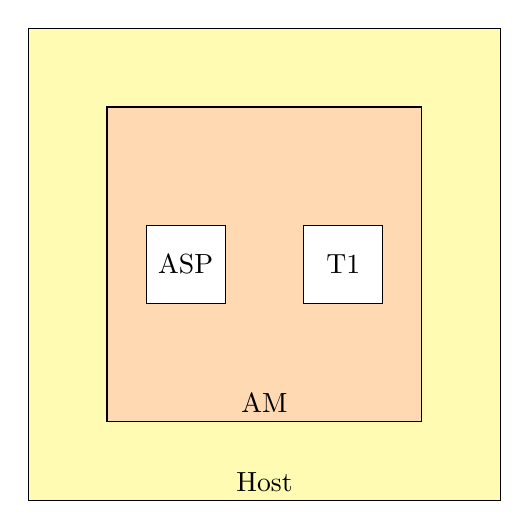
\begin{tikzpicture}
  
      \node[rectangle,
            draw,
            fill = yellow!30,
            minimum width = 6cm, 
            minimum height = 6cm] (r) at (0,0) {};
      \node[anchor=south] at (r.south) {Host};
      
      \node[rectangle,
            draw,
            fill = orange!30,
            minimum width = 4cm, 
            minimum height = 4cm] (AM) at (r.center) {};
      \node[anchor=south] at (AM.south) {AM}; 

      \node[rectangle,
            draw,
            fill = white,
            minimum width = 1cm, 
            minimum height = 1cm] (ASP) at (-1,0) {};
      \node at (ASP.center) {ASP};

      \node[rectangle,
            draw,
            fill = white,
            minimum width = 1cm, 
            minimum height = 1cm] (T1) at (1,0) {};
      \node at (T1.center) {T1};
      
      

      
  
  \end{tikzpicture}
  \caption{Total system.}
  \label{fig:System1}
\end{figure}

\end{document}